% =============================================================================
% COPYRIGHT AND DISCLAIMER
% =============================================================================
% This file is provided as a convenience template for competition participants.
% By using it, you accept full responsibility for compliance with all applicable
% copyright, licensing, and usage rules of the Association for Computing
% Machinery (ACM) and of any LaTeX packages you load (including, without
% limitation, the "acmart" document class and related ACM materials).
%
% Consult ACM's official publication, template, and copyright policies before
% using this setup for any purpose other than this competition. Do not assume
% that this template may be reused, redistributed, or submitted elsewhere
% without independently verifying ACM's current rules.
%
% Use of the "acmart" class, the "sigconf" option, or ACM-style formatting in
% this template does NOT mean that this report, this competition, its organizers,
% or any resulting PDF is sponsored, endorsed, affiliated with, or published by
% ACM. ACM trademarks and branding remain the property of ACM.
%
% Template packages live in preamble.tex.
% Citations live in main.bib. Edit this file with your paper content.
% =============================================================================

\documentclass[sigconf]{acmart}
% =============================================================================
% Template setup — participants normally do not edit this file.
% Author content belongs in main.tex; citations belong in main.bib.
% \documentclass lives in main.tex so Overleaf does not treat this file as root.
% =============================================================================

% --- Competition / non-ACM-submission friendly rights metadata -------------
\setcopyright{none}
\settopmatter{printacmref=false}
\acmConference[Kaggle Competition]{Filament Segmentation Challenge}{2026}{\href{https://www.kaggle.com/competitions/filament-segmentation-2026}{kaggle.com/competitions/filament-segmentation-2026}}
\acmBooktitle{Competition Report}
\acmDOI{}
\acmISBN{}

% --- Author guidance text --------------------------------------------------
% \guide{...} is gray italic while \guideStyletrue; omitted from the PDF if false.
% Flip the switch in main.tex after % =============================================================================
% Template setup — participants normally do not edit this file.
% Author content belongs in main.tex; citations belong in main.bib.
% \documentclass lives in main.tex so Overleaf does not treat this file as root.
% =============================================================================

% --- Competition / non-ACM-submission friendly rights metadata -------------
\setcopyright{none}
\settopmatter{printacmref=false}
\acmConference[Kaggle Competition]{Filament Segmentation Challenge}{2026}{\href{https://www.kaggle.com/competitions/filament-segmentation-2026}{kaggle.com/competitions/filament-segmentation-2026}}
\acmBooktitle{Competition Report}
\acmDOI{}
\acmISBN{}

% --- Author guidance text --------------------------------------------------
% \guide{...} is gray italic while \guideStyletrue; omitted from the PDF if false.
% Flip the switch in main.tex after % =============================================================================
% Template setup — participants normally do not edit this file.
% Author content belongs in main.tex; citations belong in main.bib.
% \documentclass lives in main.tex so Overleaf does not treat this file as root.
% =============================================================================

% --- Competition / non-ACM-submission friendly rights metadata -------------
\setcopyright{none}
\settopmatter{printacmref=false}
\acmConference[Kaggle Competition]{Filament Segmentation Challenge}{2026}{\href{https://www.kaggle.com/competitions/filament-segmentation-2026}{kaggle.com/competitions/filament-segmentation-2026}}
\acmBooktitle{Competition Report}
\acmDOI{}
\acmISBN{}

% --- Author guidance text --------------------------------------------------
% \guide{...} is gray italic while \guideStyletrue; omitted from the PDF if false.
% Flip the switch in main.tex after \input{preamble}.
%
% Do not use \guide{...} for \email{...}.
\usepackage{xcolor}
\newif\ifguideStyle
\guideStyletrue
\newcommand{\guide}[1]{%
  \ifguideStyle
    {\color{gray!65}\itshape #1}%
  \fi
}

% --- Math ------------------------------------------------------------------
% Do NOT load amssymb (or amsfonts): acmart already loads newtxmath, which
% defines the same symbols (e.g. \Bbbk) and causes a conflict on Overleaf.
% amsmath is already provided by acmart; mathtools extends it.
\usepackage{mathtools}

% --- Figures ---------------------------------------------------------------
% graphicx is already loaded by acmart
\usepackage{subcaption}

% --- Tables ----------------------------------------------------------------
% booktabs is already loaded by acmart
\usepackage{tabularx}
\usepackage{multirow}

% --- Bibliography style is set in main.tex (ACM-Reference-Format) ----------
.
%
% Do not use \guide{...} for \email{...}.
\usepackage{xcolor}
\newif\ifguideStyle
\guideStyletrue
\newcommand{\guide}[1]{%
  \ifguideStyle
    {\color{gray!65}\itshape #1}%
  \fi
}

% --- Math ------------------------------------------------------------------
% Do NOT load amssymb (or amsfonts): acmart already loads newtxmath, which
% defines the same symbols (e.g. \Bbbk) and causes a conflict on Overleaf.
% amsmath is already provided by acmart; mathtools extends it.
\usepackage{mathtools}

% --- Figures ---------------------------------------------------------------
% graphicx is already loaded by acmart
\usepackage{subcaption}

% --- Tables ----------------------------------------------------------------
% booktabs is already loaded by acmart
\usepackage{tabularx}
\usepackage{multirow}

% --- Bibliography style is set in main.tex (ACM-Reference-Format) ----------
.
%
% Do not use \guide{...} for \email{...}.
\usepackage{xcolor}
\newif\ifguideStyle
\guideStyletrue
\newcommand{\guide}[1]{%
  \ifguideStyle
    {\color{gray!65}\itshape #1}%
  \fi
}

% --- Math ------------------------------------------------------------------
% Do NOT load amssymb (or amsfonts): acmart already loads newtxmath, which
% defines the same symbols (e.g. \Bbbk) and causes a conflict on Overleaf.
% amsmath is already provided by acmart; mathtools extends it.
\usepackage{mathtools}

% --- Figures ---------------------------------------------------------------
% graphicx is already loaded by acmart
\usepackage{subcaption}

% --- Tables ----------------------------------------------------------------
% booktabs is already loaded by acmart
\usepackage{tabularx}
\usepackage{multirow}

% --- Bibliography style is set in main.tex (ACM-Reference-Format) ----------


% ---- numbers: generated by report/make_figures.py, work/make_efficiency.py and report/uncertainty.py ----
\InputIfFileExists{numbers.tex}{}{}
\InputIfFileExists{official_numbers.tex}{}{}
\InputIfFileExists{efficiency_numbers.tex}{}{}
\InputIfFileExists{uncertainty_numbers.tex}{}{}
\providecommand{\uncCILo}{--}\providecommand{\uncCIHi}{--}\providecommand{\uncRulesCILo}{--}
\providecommand{\uncRulesCIHi}{--}\providecommand{\uncFoldMean}{--}\providecommand{\uncFoldStd}{--}
\providecommand{\uncFoldMin}{--}\providecommand{\uncFoldMax}{--}\providecommand{\uncGainLo}{--}
\providecommand{\uncGainHi}{--}\providecommand{\uncGainPos}{--}\providecommand{\uncNBoot}{2{,}000}
\providecommand{\uncFoldMeanRules}{--}\providecommand{\uncFoldStdRules}{--}

% Guide styling: \guideStyletrue = show gray italic hints; \guideStylefalse = omit them
% \guideStyletrue
\guideStylefalse

\begin{document}

\title{Agreement-Aware U-Net Segmentation of Solar Filaments Optimised for Panoptic Quality}
\subtitle{A Solution to the Solar Filament Segmentation Challenge 2026} % DO NOT CHANGE


\author{Shubham Tambe}
\affiliation{%
  \country{India}
}
\email{tambeshubham2004@gmail.com}

\begin{abstract}
    This report describes our solution to the Solar Filament Segmentation Challenge~2026, a Kaggle competition on automatic segmentation of solar filaments in GONG H-$\alpha$ observations. Independent annotators of the same image agree only at a Panoptic Quality (PQ) of \humanPQ{}. We therefore train U-Net ensembles on the per-pixel fraction of annotators that mark a filament, form instances with a small rule set tuned directly for PQ, and redraw each instance with a second-stage network on rotated native-resolution crops. Validated out of fold against every annotator, the final 20-model pipeline reaches PQ~\refPQ{} (95\% bootstrap interval \uncCILo--\uncCIHi; SQ~\refSQ{}, RQ~\refRQ{}) at \effFinalT{}\,s per image on a laptop GPU, with fragmentation and over-merging close to the human level; a ten-model version reaches \effPQFastRef{} at \effTFastRef{}\,s per image.
\end{abstract}

\maketitle


% ==================================== %
%              INTRODUCTION            %
% ==================================== %
\section{Introduction}
    This report goes over the details of our submitted solution to the Solar Filament Segmentation Challenge~2026 \cite{filament-segmentation-2026}. The challenge, launched on July~10,~2026, is organized by the Earth-Space AI Research (ESAIR) Lab\footnote{\href{https://www.esairlab.com/home}{www.esairlab.com/}}. This challenge utilizes the MAGFiLO dataset for evaluation of the segmentation algorithms \cite{ahmadzadeh2024dataset}. Predictions are scored with Panoptic Quality~\cite{kirillov2019panoptic},
\begin{equation}
\mathrm{PQ}=\underbrace{\frac{\sum_{(p,g)\in TP}\mathrm{IoU}(p,g)}{|TP|}}_{\text{SQ}}\times
\underbrace{\frac{|TP|}{|TP|+\tfrac12|FP|+\tfrac12|FN|}}_{\text{RQ}},
\end{equation}
where a prediction matches a reference filament when their IoU exceeds 0.5, so both fragmentation and over-merging are penalised. Many images were labelled by several annotators independently; scoring every pair of annotators of the same image with this metric gives PQ~\humanPQ{} (SQ~\humanSQ{}, RQ~\humanRQ{}). They disagree on boundary width, on which faint filaments to include, and on whether a long filament is one instance or several, so a model scored against single annotators cannot be expected to exceed this level by much.

Earlier work segmented filaments with U-Net-style networks~\cite{ahmadzadeh2019toward}; general instance segmentation is usually solved with proposal-based detectors such as Mask R-CNN~\cite{he2017maskrcnn}. For thin, faint, multiply-annotated filaments we instead predict a probability map and form instances from it. Our contributions are (i)~training on the annotators' vote rather than on one annotator, (ii)~instance rules and a second-stage refiner tuned directly for pooled PQ, and (iii)~a fully cross-fitted validation with uncertainty estimates and an accuracy-versus-cost comparison. Our Kaggle team is \emph{shubhami9}; code, weights and an executed notebook are public~\cite{tambe2026code}.


% ==================================== %
%              METHODOLOGY             %
% ==================================== %
\section{Methodology}\label{sec:methodology}
Figure~\ref{fig:pipeline} shows the end-to-end pipeline. All components are existing, cited algorithms; our contribution is how they are trained, combined and tuned for the metric.

\begin{figure*}[t]
\centering
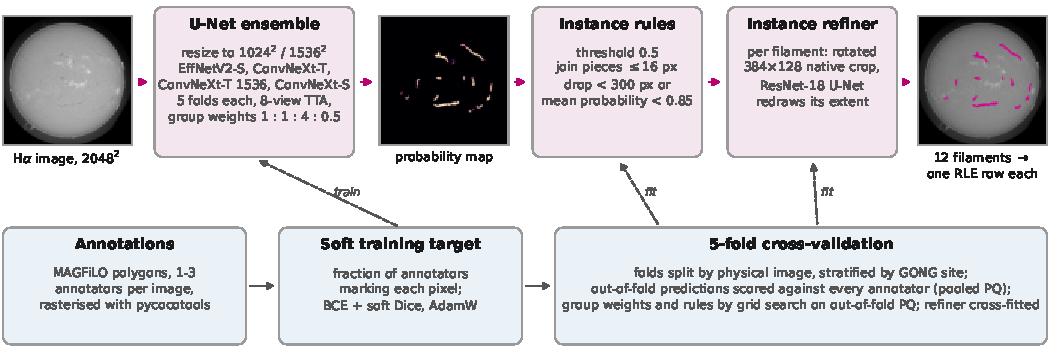
\includegraphics[width=\textwidth]{figures/pipeline.pdf}
\caption{End-to-end pipeline. Top: inference, shown on a training image with its out-of-fold probability map and its final out-of-fold instances (right). Bottom: training and validation; dashed arrows show which part each step trains or fits (on out-of-fold predictions only).}
\Description{Flow diagram from the H-alpha image through the U-Net ensemble, the probability map, the instance rules and the instance refiner to the final instances, with the training and validation steps below.}
\label{fig:pipeline}
\end{figure*}

\subsection{Data, splits and sampling}
The training set has \nImages{} physical GONG~\cite{harvey1996gong} images (2048$\times$2048) with \nSets{} annotation sets and \nFilaments{} filament polygons; \nMulti{} images were labelled by two or three annotators. Filaments are small and thin (median area $\approx$1.2k\,px, width $\approx$13\,px). We split the training images into five folds by \emph{physical image} (never by annotation set, which would leak an image into its own validation), stratified by GONG site; one model per fold is trained on the other four folds, and the out-of-fold predictions are used for all model selection and tuning. The 180 test images are used only to produce the submission. Each epoch is a shuffled pass over all training images of the fold as full-disk inputs (no patch sampling). Polygons are rasterised with pycocotools~\cite{lin2014coco}, which also computes the reference \texttt{area} field; OpenCV's \texttt{fillPoly} includes boundary pixels and makes masks 11\% larger (median), a large bias for 13-px-wide objects.

\subsection{Agreement-aware target and networks}
Rather than picking one annotator per image, the target of each pixel is the fraction of annotators that marked it ($0,\tfrac13,\tfrac12,\tfrac23,1$), i.e.\ the expected label of a randomly chosen annotator. The loss is binary cross-entropy (which accepts soft targets) plus a batch soft-Dice term~\cite{milletari2016vnet} against the class imbalance (filaments cover $\approx$0.3\% of the disk).

The networks are U-Nets~\cite{ronneberger2015unet} from segmentation\_models\_pytorch~\cite{iakubovskii2019smp} with ImageNet-pretrained timm~\cite{wightman2019timm} encoders: EfficientNetV2-S~\cite{tan2021efficientnetv2} and ConvNeXt-T~\cite{liu2022convnext} at 1024\,px, ConvNeXt-T at 1536\,px and ConvNeXt-S at 1024\,px. They take the full disk resized to that size (one grayscale channel; filaments are $\approx$6\,px wide at 1024\,px) and output one logit per pixel. Augmentations: any rotation about the disk centre, flips, $\pm$10\% scale (the disk radius varies by about 10\% across sites), small shifts, brightness/contrast/gamma, occasional blur and noise. We train for 40 epochs (30 at 1536\,px) with AdamW~\cite{loshchilov2019adamw} (weight decay $10^{-4}$, one warm-up epoch, cosine decay; learning rate $5\!\times\!10^{-4}$ with batch 4 for EfficientNetV2-S, $2.5\!\times\!10^{-4}$ (ConvNeXt-T) or $2\!\times\!10^{-4}$ (ConvNeXt-S) with batch 2) in mixed precision. One fold takes 45--120 minutes on an 8\,GB RTX~3070~Ti Laptop GPU or a free Kaggle T4. Encoders whose pretrained weights are licensed for non-commercial use only (e.g.\ SegFormer/MiT) were not used.

\subsection{Inference and instance formation}
Each model averages the eight symmetric views of the image (flips $\times$ transpose; +0.002 PQ over four flips), the five fold models of a family are averaged, and the four families are blended with weights 1\,:\,1\,:\,4\,:\,0.5 (EfficientNetV2-S, ConvNeXt-T 1024, ConvNeXt-T 1536, ConvNeXt-S), chosen by a joint grid search on out-of-fold PQ. The blended map is turned into instances by three rules:
\begin{enumerate}
\item threshold at $\ppThreshold$;
\item blobs separated by at most $\ppMergeGap$\,px form one filament: background pixels within half that distance of a blob bridge blobs in a connectivity pass, but each instance keeps only its own pixels, so grouping does not thicken masks;
\item drop instances smaller than $\ppMinArea$\,px or with mean probability below $\ppMinMeanProb$, keeping the most confident region if an image would otherwise be empty.
\end{enumerate}
The four values maximise pooled out-of-fold PQ in a grid search (candidates are scored from foreground pixels only, so a 1{,}000-point grid takes minutes).

\subsection{Instance refinement}
A threshold of one probability map cannot always reproduce the extent annotators draw (filaments cut short, merged with a neighbour, drawn thinner). Each instance from the rules is therefore re-segmented in its own crop, rotated so that the filament's long axis is horizontal, covering 150\% of its length and never up-sampled ($384\times128$ native pixels). A small U-Net (ResNet-18 encoder~\cite{he2016resnet}) receives four channels (image, ensemble probability, the instance's own mask, the masks of the other instances) and predicts the consensus of the annotators who drew the matching filament. The refined probability is warped back and each pixel goes to the instance with the highest refined probability above 0.5. Existence is still decided by the rules; only the extent changes. The idea follows a public notebook~\cite{dud2026}; the implementation is our own. The refiner is cross-fitted: the one applied to fold $k$ never saw crops of fold $k$.

\begin{figure}[t]
\centering
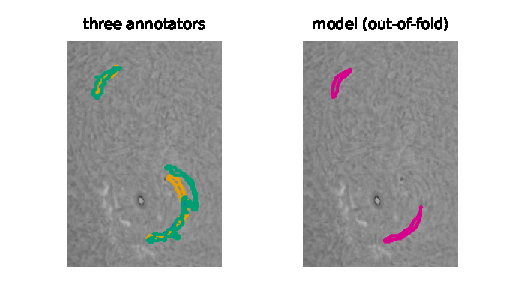
\includegraphics[width=\columnwidth]{figures/qualitative.pdf}
\caption{Example segmentation: a validation image labelled by three annotators (left, one colour each) and the out-of-fold prediction of the tuned rules (right). Annotators differ in width, extent and splitting much as the model does.}
\Description{Two crops of the same solar region: three annotators' filament outlines on the left and the model's outlines on the right.}
\label{fig:qual}
\end{figure}


% ==================================== %
%              EVALUATION              %
% ==================================== %
\section{Evaluation}\label{sec:evaluation}
\subsection{Evaluation strategy}
Every out-of-fold prediction is scored against \emph{every} annotator of its image with the competition's PQ definition, and the statistics (summed matched IoU, TP, FP, FN) are pooled over all image--annotator pairs, which rewards predicting what a typical annotator draws. We also run the organisers' self-evaluation analysis (IoU and Dice distributions, one-to-many and many-to-one cases). Uncertainty is reported in two ways: the spread of PQ over the five folds, and 95\% bootstrap intervals from \uncNBoot{} resamples of the \nOOF{} images (pooled PQ recomputed for each resample; paired for differences).

\begin{table}[t]
\centering
\caption{Out-of-fold results on \nOOF{} training images, scored against every annotator, with 95\% bootstrap intervals of PQ.}
\label{tab:main}
\begin{tabular}{@{}lcccc@{}}
\toprule
 & PQ & 95\% interval & SQ & RQ \\
\midrule
Annotator vs.\ annotator & \humanPQ & -- & \humanSQ & \humanRQ \\
Ensemble, threshold 0.5 & \defPQ & -- & \defSQ & \defRQ \\
Ensemble, decision layer & \decPQ & -- & \decSQ & \decRQ \\
Ensemble, tuned rules & \cvPQ & \uncRulesCILo--\uncRulesCIHi & \cvSQ & \cvRQ \\
\quad + refiner (final) & \textbf{\refPQ} & \uncCILo--\uncCIHi & \refSQ & \refRQ \\
\bottomrule
\end{tabular}
\end{table}

\subsection{Results}
Table~\ref{tab:main} summarises the results. Forming instances for PQ mainly raises recognition quality: false positives fall from \defFP{} (single threshold) to \cvFP{} and fragmented filaments from \defOneToMany{} to \cvOneToMany{}, while SQ is essentially unchanged. The refiner then improves both SQ and RQ. Over the five folds the final pipeline reaches PQ \uncFoldMean{}\,$\pm$\,\uncFoldStd{} (mean\,$\pm$\,standard deviation; range \uncFoldMin--\uncFoldMax), and the paired bootstrap interval of the refiner's gain over the rules is \uncGainLo{} to \uncGainHi{} (positive in \uncGainPos\% of resamples). Even the lower end of the interval lies far above the human agreement of \humanPQ{}.

\textbf{Organisers' analysis.} Re-running the organisers' self-evaluation analysis on the out-of-fold predictions of the tuned rules (Fig.~\ref{fig:dist}) reproduces our PQ exactly (\offModelPQ{}). Over all overlapping reference--prediction pairs the mean IoU is \offModelIoU{} (two annotators: \offHumanIoU{}) and the mean Dice \offModelDice{} (\offHumanDice{}). Fragmentation stays close to the human level: \offModelSplit\% of reference filaments overlap two or more predictions (annotators: \offHumanSplit\%) and \offModelMerge\% of predictions overlap two or more reference filaments (\offHumanMerge\%). Our instances never overlap, so every reference filament can match at most one prediction, as in the original PQ definition~\cite{kirillov2019panoptic}.

\begin{figure*}[t]
\centering
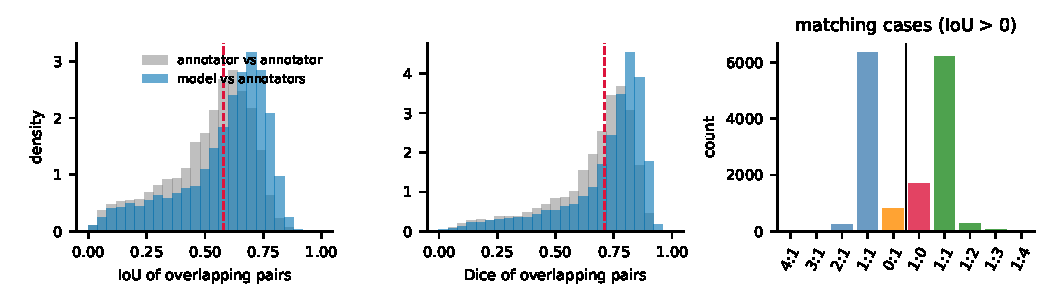
\includegraphics[width=\textwidth]{figures/official_eval.pdf}
\caption{Organisers' self-evaluation analysis, out of fold (\nOOF{} images). Left, centre: IoU and Dice of all overlapping reference--prediction pairs for the model (blue, dashed line = mean) and between two annotators (grey). Right: matching cases; 1:$n$ = a reference filament overlapped by $n$ predictions, $n$:1 = a prediction overlapping $n$ reference filaments, 1:0 / 0:1 = misses.}
\Description{Histograms of IoU and Dice for the model and for annotator pairs, and a bar chart of one-to-many and many-to-one matching cases.}
\label{fig:dist}
\end{figure*}

\textbf{Where errors come from.} Recall is \recallLarge{} for filaments of at least 600\,px but only \recallSmall{} below (Fig.~\ref{fig:size}); small filaments are also where annotators disagree most. Of the missed reference filaments, \nearMissShare{} are near misses (best IoU 0.25--0.5): the filament was found but drawn with a different extent or split differently, mirroring the human disagreement. Precision rises steeply with the mean probability of an instance, which is why the confidence filter is the most effective rule.

\begin{figure}[t]
\centering
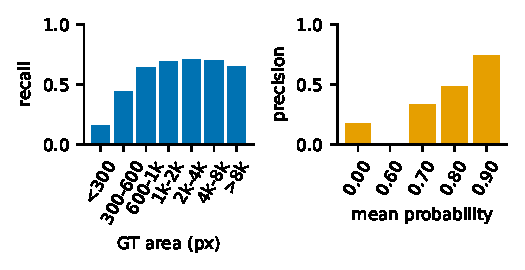
\includegraphics[width=\columnwidth]{figures/size_confidence.pdf}
\caption{Recall by reference filament area and precision by instance confidence (out of fold).}
\Description{Bar charts: recall rises with filament area; precision rises with mean instance probability.}
\label{fig:size}
\end{figure}

\textbf{A PQ-optimal decision layer (analysis).} Every predicted instance adds exactly $\tfrac12$ to the PQ denominator, matched or not, so the optimal submission keeps exactly the candidates whose annotator-expected matched IoU exceeds $\mathrm{PQ}^*/2$ (Dinkelbach~\cite{dinkelbach1967}). We built candidates at 17 thresholds, scored them with cross-fitted gradient-boosted trees and selected the best non-overlapping set exactly by dynamic programming over the candidate forest (idea from~\cite{dud2026}, implementation our own). It reaches PQ~\decPQ{} against \cvPQ{} for the tuned rules, a tie within noise, so we submit the simpler rules.

\begin{table}[t]
\centering
\caption{Out-of-fold PQ vs.\ end-to-end inference time per 2048$\times$2048 image (\effGPU{}, 8-view TTA).}
\label{tab:cost}
\begin{tabularx}{\columnwidth}{@{}Xrrr@{}}
\toprule
Pipeline & Models & s/image & PQ \\
\midrule
% BEGIN efficiency rows (generated by work/make_efficiency.py)
ResNet-34, 1024\,px, rules & 5 & 1.1 & 0.418 \\
ResNet-34 + UNet++, refiner & 20 & 10.5 & 0.435 \\
\quad + EffNetV2-S + ConvNeXt-T & 30 & 13.6 & 0.438 \\
EffNetV2-S + ConvNeXt-T, rules & 10 & 3.2 & 0.434 \\
\quad + refiner (fast mode) & 10 & 3.7 & 0.442 \\
\quad + ConvNeXt-T 1536 + ConvNeXt-S (final) & 20 & 8.6 & \textbf{0.443} \\
% END efficiency rows
\bottomrule
\end{tabularx}
\end{table}

\textbf{Accuracy and compute.} Table~\ref{tab:cost} measures the end-to-end cost per image on one laptop GPU, rules and refiner included. Accuracy saturates quickly: ten 1024-px models of two modern encoder families (EfficientNetV2-S, ConvNeXt-T) with the refiner are more accurate than a 30-model ensemble that adds ResNet-34~\cite{he2016resnet} U-Nets and UNet++~\cite{zhou2018unetpp} models, at a quarter of the cost. The final pipeline adds two ConvNeXt groups for a further +0.001; the ten-model pipeline is the choice when compute matters. Dropping test-time augmentation makes every row about five times faster. On the public leaderboard the scores rose in the same order, from 0.34 for a single model to 0.39 for the final pipeline; all choices were made on out-of-fold PQ only.

\subsection{Strengths, weaknesses and improvements}
\textbf{Strengths.} The pipeline exceeds the agreement between two annotators by a wide margin, with fragmentation and over-merging at the human level; its post-processing is three interpretable rules; every number is out of fold and cross-fitted; a ten-model mode gives almost the same PQ at 3.7\,s per image.
\textbf{Weaknesses.} Small filaments are often missed (recall \recallSmall{} below 600\,px), and a third of the misses are near misses whose extent or splitting differs from the annotator's. The ensemble with 8-view TTA is heavy for real-time use, and the public score (0.39, about 90 images) lies below the out-of-fold PQ, within the noise of so few images.
\textbf{Improvements.} Higher input resolution for small filaments, explicit instance cues learned from the masks (e.g.\ a predicted filament axis) to decide splitting and merging, confidence calibration across annotators, and distilling the ensemble into a single network for speed.

\section{Code and Reproducibility}
Code (MIT licence), the trained weights of the submitted pipeline, pinned \texttt{requirements.txt} and an executed notebook that runs the full pipeline are at \url{https://github.com/Shubham-Tambei9/filament-segmentation-2026}~\cite{tambe2026code}. Training used only the official training images and their segmentation masks (no spines, boxes or class labels), with no external annotations or leaderboard probing. Running the notebook on a Kaggle T4 reproduced the out-of-fold PQ (\refRulesPQ{} rules, \refPQ{} refined) exactly.


% ==================================== %
%            ACKNOWLEDGMENT            %
% ==================================== %
\section{Acknowledgment}\label{sec:acknowledgment}
    % Do not change
    The organization of the Filament Segmentation Challenge 2026 is partially supported by the U.S. National Science Foundation (NSF) under Grant No. 2209912 and 2433781, directorate for Computer and Information Science and Engineering (CSE), and Office of Advanced Cyberinfrastructure (OAC), and Grant No. 2511630, AST Division Of Astronomical Sciences and MPS Directorate for Mathematical and Physical Sciences.

    The Filament Segmentation Challenge 2026 is sponsored by the U.S. National Science Foundation (NSF) National Solar Observatory (NSO).

    This work utilizes GONG data obtained by the NSO Integrated Synoptic Program, managed by the National Solar Observatory, which is operated by the Association of Universities for Research in Astronomy (AURA), Inc. under a cooperative agreement with the National Science Foundation and with contribution from the National Oceanic and Atmospheric Administration. The GONG network of instruments is hosted by the Big Bear Solar Observatory, High Altitude Observatory, Learmonth Solar Observatory, Udaipur Solar Observatory, Instituto de Astrofísica de Canarias, and Cerro Tololo Interamerican Observatory.

\bibliographystyle{ACM-Reference-Format}
\bibliography{main}

\end{document}
